\documentclass[a4paper]{article}

\hoffset=-1in
\voffset=-1in
\textwidth=175mm
\textheight=200mm

\usepackage{amsmath}
\usepackage{graphicx}
\usepackage{multicol}

\begin{document}
    \begin{figure}
        \centering
        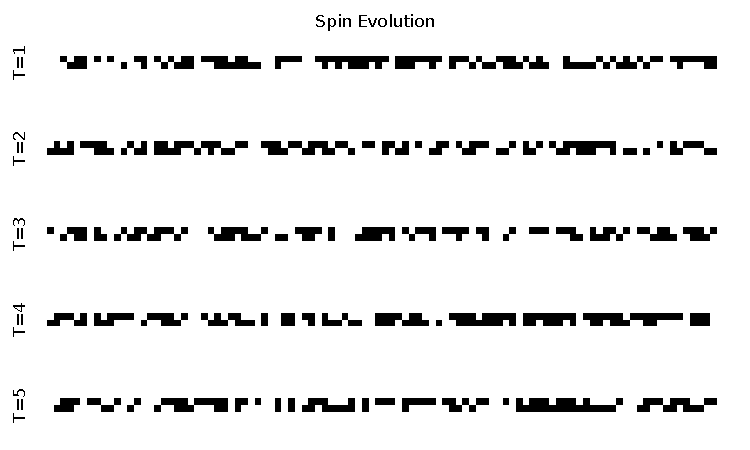
\includegraphics[width=0.5\textwidth]{pub/figures/q1a.pdf}
        \caption{At low temperatures we observed smaller groups of aligned %
            spins. We concluded that the influence of the heat (i.e. %
            \(\tau\sigma\)) on the free energy was low and therefore, that %
            the energy \(U\) was minmised.}
        \label{FIG1}
    \end{figure}

    \begin{multicols}{2}
        Given the partition function \(Z = (2\cosh(\epsilon / \tau))^{N}\), we 
        calculated the internal energy using,
        %
        \begin{align}
            U &= \tau^{2}\partial_{\tau}\ln(Z) \\
                &= \tau^{2}\partial_{\tau}
                    \ln\left(2\cosh\left(\frac{\epsilon}{\tau}\right)^{N}\right)
                    \nonumber \\
                &= N\tau^{2}\partial_{\tau}
                    \ln\left(2\cosh\left(\frac{\epsilon}{\tau}\right)\right)
                    \nonumber \\
                &= N\tau^{2}\partial_{\tau}
                    \left(2\cosh\left(\frac{\epsilon}{\tau}\right)\right)
                    \frac{1}{2\cosh\left(\frac{\epsilon}{\tau}\right)}
                    \nonumber \\
                &= N\tau^{2}\partial_{\tau}\left(\frac{\epsilon}{\tau}\right)
                    \frac{\sinh\left(\frac{\epsilon}{\tau}\right)}
                    {\cosh\left(\frac{\epsilon}{\tau}\right)}\nonumber \\
                &= -\epsilon N\tanh\left(\frac{\epsilon}{\tau}\right). 
        \end{align}
        %
        We calculated the free energy of the system using,
        %
        \begin{align}
            F &= -\tau\ln Z \\
                &= 
    \end{multicols}
\end{document}
